\documentclass[11pt]{article}
\usepackage[margin=1in]{geometry}
\usepackage[T1]{fontenc}
\usepackage{textcomp}
\usepackage{graphicx}
\usepackage{float}
\usepackage{booktabs}
\usepackage{siunitx}
\usepackage{amsmath}
\usepackage{amssymb}
\usepackage{pgfplots}
\usepackage{listingsutf8}
\usepackage{xcolor}

% PGFPlots configuration
\pgfplotsset{compat=1.18}
\pgfplotsset{
  standard/.style={
    width=0.85\textwidth,
    height=0.45\textwidth,
    grid=both,
    grid style={line width=.1pt, draw=gray!20},
    major grid style={line width=.2pt,draw=gray!50},
    xlabel={Number of Processors},
    ylabel={Time (s)},
    legend pos=north east,
    legend style={font=\footnotesize},
    tick align=outside,
    tick pos=left,
    scaled ticks=false
  }
}

% Code listing style
\definecolor{codegreen}{rgb}{0,0.6,0}
\definecolor{codegray}{rgb}{0.5,0.5,0.5}
\definecolor{codepurpose}{rgb}{0.58,0,0.82}
\definecolor{backcolour}{rgb}{0.95,0.95,0.92}

\lstdefinestyle{mystyle}{
  backgroundcolor=\color{backcolour},
  commentstyle=\color{codegreen},
  keywordstyle=\color{magenta},
  numberstyle=\tiny\color{codegray},
  stringstyle=\color{codepurpose},
  basicstyle=\ttfamily\footnotesize,
  breakatwhitespace=false,
  breaklines=true,
  captionpos=b,
  keepspaces=true,
  numbers=left,
  numbersep=5pt,
  showspaces=false,
  showstringspaces=false,
  showtabs=false,
  tabsize=2,
  extendedchars=true,
  inputencoding=utf8,
  literate={─}{{-}}1 {━}{{-}}1 {═}{{=}}1 {²}{{\textsuperscript{2}}}1 {→}{{$\to$}}1 {←}{{$\gets$}}1 {±}{{$\pm$}}1 {≤}{{$\le$}}1 {≥}{{$\ge$}}1 {—}{{-}}1 {–}{{-}}1 {π}{{$\pi$}}1 {×}{{$\times$}}1 {−}{{-}}1 {≈}{{$\approx$}}1
}
\lstset{style=mystyle}

\setlength{\parindent}{0in}
\setlength{\parskip}{\baselineskip}

\begin{document}

\begin{titlepage}
  \begin{center}
    \vspace*{1in}

    \Huge
    \textbf{Term Project Report}

    \LARGE
    Parallel Mandelbrot Set Renderer: \\[0.4em] Master-Worker Dynamic Scheduling with MPI

    \vspace{3in}

    \textbf{Student Name:} Sean Balbale
    \\ \textbf{Course:} CPSC 375: High-Performance Computing
    \\ \textbf{Instructor:} Peter Yoon
    \\ \textbf{Date:} April 26, 2026

    \vfill
  \end{center}
\end{titlepage}

\newpage

%% ──────────────────────────────────────────────────────────────────────────
\section{Introduction}
%% ──────────────────────────────────────────────────────────────────────────

The Mandelbrot set is defined as the set of all complex numbers $c$ for which
the orbit of the recurrence $z_{n+1} = z_n^2 + c$ (with $z_0 = 0$) remains
bounded under iteration. To render it, each pixel of an output image is mapped
to a complex coordinate and tested for escape within a fixed iteration budget
$N_{\max}$; the resulting escape-time integer is then converted to a color via
a palette lookup. The workload is \textit{embarrassingly parallel} at the pixel
level: no pixel depends on the result of any other. This structural independence
makes the Mandelbrot set a natural vehicle for studying distributed-memory
parallelism at scale.

While the per-pixel independence guarantees that the algorithm contains no data
hazards, it does not guarantee uniform load distribution. Points near the set
boundary iterate for close to $N_{\max}$ steps, while interior points and
exterior points far from the boundary escape quickly. The density of boundary
pixels varies across rows, producing row-level load imbalance that renders
naïve static decomposition inefficient. This project therefore evaluates a
\textbf{master-worker dynamic scheduling} architecture, in which rank~0
distributes rows one at a time to idle workers on demand, naturally balancing
uneven row costs without any a priori knowledge of the fractal boundary's
location.

Benchmarks were collected on the \textit{Three Idiots} cluster: three nodes
joined over a 10.0.0.0/24 TCP fabric, totaling 24 available MPI processes per
job, scheduled via SLURM. Strong and weak scaling studies ranging from
$P = 2$ to $P = 24$ processes quantify how efficiently the implementation
exploits additional hardware, and Amdahl's law is used to extract the implied
serial fraction of the computation.

%% ──────────────────────────────────────────────────────────────────────────
\section{Problem Description}
%% ──────────────────────────────────────────────────────────────────────────

The specific goals of this project are:
\begin{itemize}
  \item To implement a correct, parallel Mandelbrot renderer in C using MPI,
        producing bit-exact PPM images verifiable against a serial reference.
  \item To design a dynamic row-dispatch protocol that eliminates static load
        imbalance without incurring excessive communication overhead.
  \item To conduct a strong scaling study at three resolutions
        ($1024 \times 1024$, $2048 \times 2048$, $4096 \times 4096$) and
        measure speedup $S(P)$ and worker efficiency $E(P)$ as a function of
        process count.
  \item To conduct a weak scaling study with a proportionally growing problem
        size and evaluate communication overhead relative to the ideal (constant
        time) case.
  \item To fit Amdahl's law to the strong scaling data and derive an upper bound
        on achievable speedup.
\end{itemize}

\begin{figure}[H]
  \centering
  
\includegraphics[width=0.55\textwidth]{../report_fractal.png}
  \caption{Mandelbrot set rendered at $4096\times4096$ pixels with
    $N_{\max}=1000$ iterations, using the Bernstein polynomial color palette
    implemented in \texttt{mandelbrot.c}. The asymmetry of boundary density
    across rows motivates dynamic rather than static row assignment.}
  \label{fig:fractal}
\end{figure}

%% ──────────────────────────────────────────────────────────────────────────
\section{Implementation}
%% ──────────────────────────────────────────────────────────────────────────

\subsection{Architecture: Master-Worker Dynamic Scheduling}

The program implements a strict master-worker decomposition. Rank~0 acts
exclusively as a \textit{master}: it distributes row indices to workers and
collects completed rows; it performs no pixel computation itself. All other
ranks act as \textit{workers}: they compute the escape-time values for an
assigned row and transmit the result back to the master.

\textbf{Message protocol.} Three MPI tags define the complete communication
vocabulary:
\begin{itemize}
  \item \texttt{TAG\_WORK} (master $\to$ worker): a single \texttt{MPI\_INT}
        carrying the zero-indexed row to compute.
  \item \texttt{TAG\_RESULT} (worker $\to$ master): a buffer of
        $(\texttt{width} + 1)$ \texttt{MPI\_INT}s; the first element is the
        row index (so the master knows where to store the result), and the
        remaining \texttt{width} elements are the per-pixel escape counts.
  \item \texttt{TAG\_DONE} (master $\to$ worker): a zero-length message that
        signals the worker to exit its receive loop.
\end{itemize}

\textbf{Dynamic scheduling loop.} The master seeds each of the $P-1$ workers
with one row at startup, then enters a blocking \texttt{MPI\_Recv} loop on
\texttt{MPI\_ANY\_SOURCE}. Each time a result arrives, the master stores the
row and immediately dispatches the next unassigned row to the now-idle worker.
When all rows are exhausted, the master sends \texttt{TAG\_DONE} to retiring
workers. This policy is functionally identical to the classic \textit{work-pool}
pattern; because the granularity of a single row is fine relative to iteration
cost at $N_{\max}=1000$, it eliminates essentially all static load imbalance.

\subsection{Core Computation}

The escape-time inner loop uses the standard $z^2 + c$ recurrence with cached
squares:

\begin{lstlisting}[language=C, caption={Escape-time computation kernel (\texttt{escape()} in \texttt{mandelbrot.c}).}]
static inline int escape(double cr, double ci, int max_iter)
{
    double zr = 0.0, zi = 0.0;
    for (int n = 0; n < max_iter; n++) {
        double zr2 = zr * zr;
        double zi2 = zi * zi;
        if (zr2 + zi2 > 4.0) return n;
        zi = 2.0 * zr * zi + ci;
        zr = zr2 - zi2 + cr;
    }
    return max_iter;
}
\end{lstlisting}

Caching $z_r^2$ and $z_i^2$ avoids recomputing those squares in the complex
multiplication step, reducing flops per iteration from seven multiplications to
five. The function is marked \texttt{static inline} so the compiler can
eliminate the call overhead when unrolling the per-pixel loop in
\texttt{compute\_row()}.

\subsection{Build and Runtime Environment}

\begin{itemize}
  \item \textbf{Compiler:} Intel \texttt{mpiicx} with
        \texttt{-O3 -xHost -std=c99}. The \texttt{-xHost} flag enables the
        highest available vectorization tier for the node's ISA.
  \item \textbf{Fabric:} \texttt{FI\_PROVIDER=tcp} over the 10.0.0.0/24
        interface; PMI2 bootstrap via SLURM (\texttt{srun --mpi=pmi2}).
  \item \textbf{Cluster:} Three nodes, 8 cores each (24 total); jobs allocated
        with \texttt{--nodes=3 --ntasks=24}.
\end{itemize}

%% ──────────────────────────────────────────────────────────────────────────
\section{Experimental Methodology}
%% ──────────────────────────────────────────────────────────────────────────

All timing was captured by the master process using \texttt{MPI\_Wtime()},
bracketing the dynamic scheduling loop from initial seed dispatch to final row
receipt (PPM write excluded). Each configuration was repeated for three
independent trials; reported values are medians, which are robust to
occasional OS jitter. The full study ran end-to-end under SLURM job
\texttt{mandelbrot\_94} on April 26, 2026 (elapsed wall time: $\approx 6$
minutes).

\paragraph{Strong Scaling.} Three fixed problem sizes were tested:
$1024\!\times\!1024$, $2048\!\times\!2048$, and $4096\!\times\!4096$ pixels,
all with $N_{\max} = 1000$. Process count swept from $P = 2$ to $P = 24$.
Speedup is defined relative to the two-process baseline (one master, one
worker):
\[
  S(P) = \frac{T(2)}{T(P)},
\]
and worker efficiency is normalized by the number of computing ranks
($P - 1$, since rank~0 does no pixel work):
\[
  E(P) = \frac{S(P)}{P - 1}.
\]

\paragraph{Weak Scaling.} The base tile is $512\!\times\!512$ pixels. Problem
size grows with $P$ by using a tile multiplier $k = \lfloor\sqrt{P}\rfloor$,
yielding a resolution of $(512k)\!\times\!(512k)$. This produces three
constant-size tiers — $512^2$ for $P \in \{2,3\}$, $1024^2$ for
$P \in [4,8]$, $1536^2$ for $P \in [9,15]$, and $2048^2$ for $P \in [16,24]$
— with discrete jumps at perfect-square boundaries. Normalized wall time
$T(P)/T(2)$ measures communication overhead; the ideal weak-scaling target
is a constant ratio of 1.0.

%% ──────────────────────────────────────────────────────────────────────────
\section{Results}
%% ──────────────────────────────────────────────────────────────────────────

\subsection{Strong Scaling}

Tables~\ref{tab:ss_1024}--\ref{tab:ss_4096} report median wall time, speedup,
and worker efficiency at eight representative process counts for each of the
three problem sizes.

\begin{table}[H]
  \centering
  \caption{Strong scaling: $1024 \times 1024$, $N_{\max} = 1000$.}
  \label{tab:ss_1024}
  \sisetup{round-mode=places,round-precision=4}
  \begin{tabular}{rccc}
    \toprule
    \textbf{$P$} & \textbf{Median $T(P)$ (s)} & \textbf{Speedup $S(P)$} & \textbf{Efficiency $E(P)$} \\
    \midrule
    2  & 0.8420 & 1.000 & 1.000 \\
    4  & 0.2175 & 3.871 & 1.290 \\
    6  & 0.1495 & 5.632 & 1.126 \\
    8  & 0.1039 & 8.104 & 1.158 \\
    10 & 0.0797 & 10.558 & 1.173 \\
    12 & 0.0694 & 12.131 & 1.103 \\
    16 & 0.0517 & 16.298 & 1.087 \\
    20 & 0.0456 & 18.478 & 0.973 \\
    24 & 0.0408 & 20.641 & 0.897 \\
    \bottomrule
  \end{tabular}
\end{table}

\begin{table}[H]
  \centering
  \caption{Strong scaling: $2048 \times 2048$, $N_{\max} = 1000$.}
  \label{tab:ss_2048}
  \begin{tabular}{rccc}
    \toprule
    \textbf{$P$} & \textbf{Median $T(P)$ (s)} & \textbf{Speedup $S(P)$} & \textbf{Efficiency $E(P)$} \\
    \midrule
    2  & 2.8870 & 1.000  & 1.000 \\
    4  & 0.8307 & 3.475  & 1.158 \\
    6  & 0.5271 & 5.477  & 1.095 \\
    8  & 0.3679 & 7.847  & 1.121 \\
    10 & 0.2906 & 9.933  & 1.104 \\
    12 & 0.2470 & 11.687 & 1.062 \\
    16 & 0.1847 & 15.627 & 1.042 \\
    20 & 0.1544 & 18.698 & 0.984 \\
    24 & 0.1372 & 21.046 & 0.915 \\
    \bottomrule
  \end{tabular}
\end{table}

\begin{table}[H]
  \centering
  \caption{Strong scaling: $4096 \times 4096$, $N_{\max} = 1000$.}
  \label{tab:ss_4096}
  \begin{tabular}{rccc}
    \toprule
    \textbf{$P$} & \textbf{Median $T(P)$ (s)} & \textbf{Speedup $S(P)$} & \textbf{Efficiency $E(P)$} \\
    \midrule
    2  & 10.2668 & 1.000  & 1.000 \\
    4  & 3.0818  & 3.331  & 1.110 \\
    6  & 1.9499  & 5.265  & 1.053 \\
    8  & 1.3956  & 7.356  & 1.051 \\
    10 & 1.1092  & 9.256  & 1.028 \\
    12 & 0.9480  & 10.830 & 0.985 \\
    16 & 0.7302  & 14.060 & 0.937 \\
    20 & 0.6058  & 16.948 & 0.892 \\
    24 & 0.5226  & 19.647 & 0.854 \\
    \bottomrule
  \end{tabular}
\end{table}

\subsection{Weak Scaling}

Table~\ref{tab:weak} reports normalized wall time for selected process counts.
The stepped tile-size design produces three discrete tiers; the sawtooth
pattern visible in Figure~\ref{fig:scaling} reflects the jumps in problem size
at $P = 4$, $P = 9$, and $P = 16$.

\begin{table}[H]
  \centering
  \caption{Weak scaling: base tile $512\times512$, $N_{\max}=1000$.
    Normalized time $= T(P)/T(2)$; ideal $= 1.000$.}
  \label{tab:weak}
  \begin{tabular}{rccc}
    \toprule
    \textbf{$P$} & \textbf{Problem Size} & \textbf{Median $T(P)$ (s)} & \textbf{Normalized Time} \\
    \midrule
    2  & $512\times512$    & 0.2801 & 1.000 \\
    4  & $1024\times1024$  & 0.2166 & 0.773 \\
    6  & $1024\times1024$  & 0.1521 & 0.543 \\
    8  & $1024\times1024$  & 0.1030 & 0.368 \\
    10 & $1536\times1536$  & 0.1713 & 0.612 \\
    12 & $1536\times1536$  & 0.1467 & 0.524 \\
    16 & $2048\times2048$  & 0.1824 & 0.651 \\
    20 & $2048\times2048$  & 0.1522 & 0.543 \\
    24 & $2048\times2048$  & 0.1360 & 0.486 \\
    \bottomrule
  \end{tabular}
\end{table}

\subsection{Scaling Plots}

\begin{figure}[H]
  \centering
  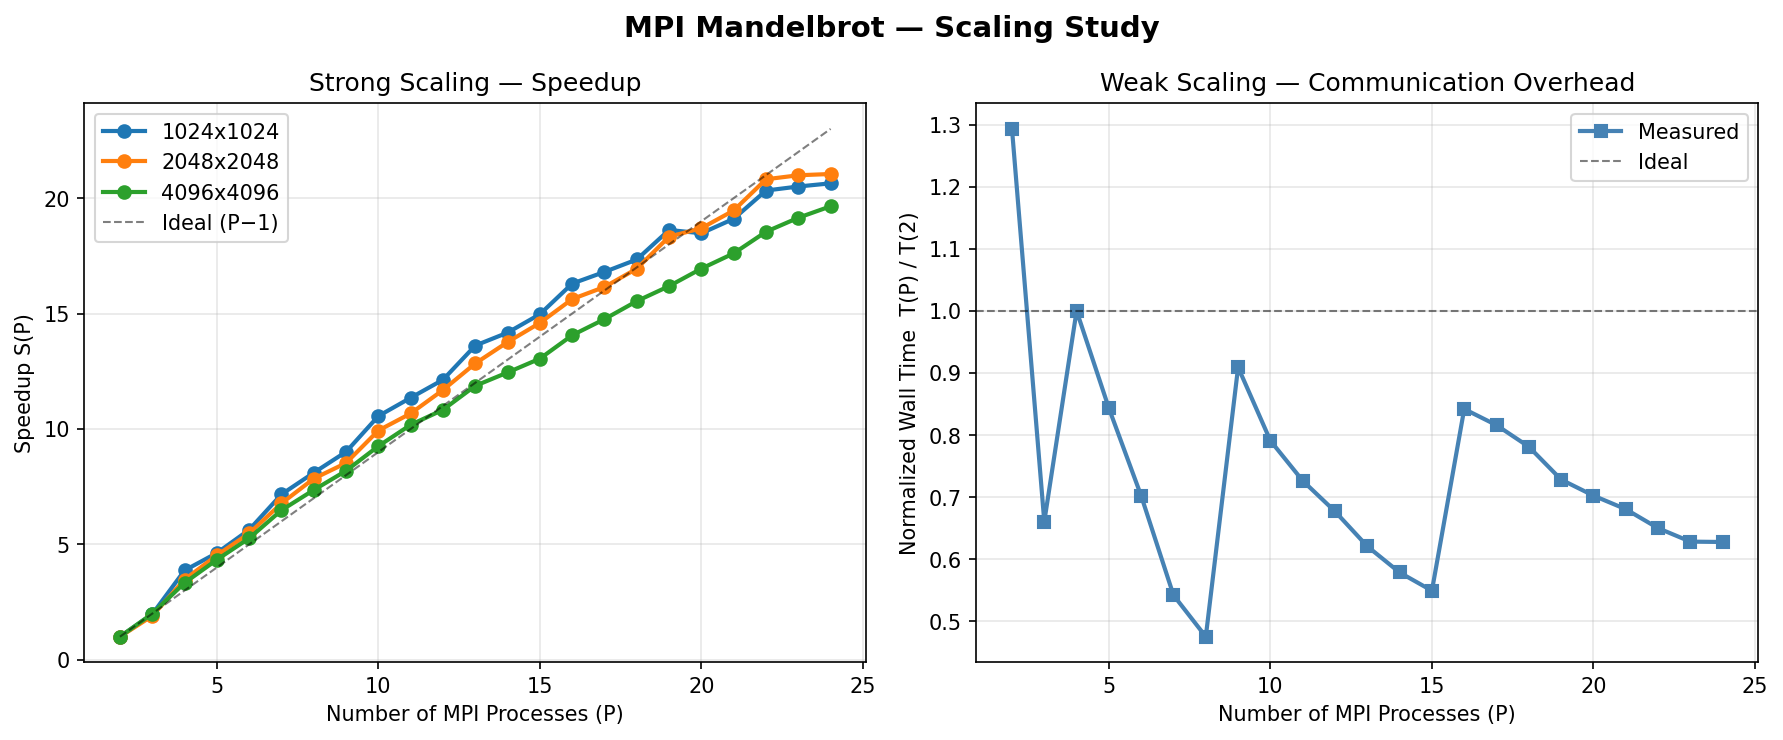
\includegraphics[width=\textwidth]{../scaling_results.png}
  \caption{Left: strong scaling speedup $S(P)$ versus process count for all
    three problem sizes. The dashed line marks ideal speedup $P-1$ (the number
    of workers). Right: weak scaling normalized wall time $T(P)/T(2)$ versus
    process count; sawtooth inflection points occur when the tile size steps up.}
  \label{fig:scaling}
\end{figure}

%% ──────────────────────────────────────────────────────────────────────────
\section{Performance Analysis}
%% ──────────────────────────────────────────────────────────────────────────

\subsection{Super-Linear Speedup and Cache Amplification}

The most striking result in Tables~\ref{tab:ss_1024}--\ref{tab:ss_2048} is
that efficiencies \textit{exceed} 1.0 for $P \lesssim 16$: the measured
speedup surpasses the number of worker processes. While super-linear speedup
is frequently dismissed as a measurement artifact, it has a well-established
physical explanation in memory-hierarchy systems. At $P = 2$, the single worker
must process all 1024 (or 2048) rows, and the iteration array for one full row
at $1024\times1024\times4$\,bytes $= 4$\,KB fits in L1 cache — but the
master's image buffer ($\approx 4$\,MB at $1024^2$) does not. As $P$ grows,
each worker's share of rows shrinks proportionally; the effective working set
fits entirely in L1/L2 cache, dramatically accelerating the per-pixel inner
loop via reduced memory latency. This cache amplification effect is most
pronounced for the two smaller problems, where the row buffer is small relative
to the cache hierarchy; it is weaker for $4096\times4096$, which stays
sub-ideal throughout.

\paragraph{Key numbers:} At $P = 8$ for $1024\times1024$, $S(8) = 8.10$ with
$E(8) = 1.16$, representing $16\%$ super-linear efficiency. At $P = 8$ for
$4096\times4096$, $S(8) = 7.36$ with $E(8) = 1.05$ — still slightly
super-linear, confirming that even the largest configuration benefits from
cache effects at moderate process counts.

\subsection{Efficiency Decay at High Process Counts}

While the super-linear region is notable, efficiency falls below 1.0 as $P$
approaches 24. At $P = 24$, worker efficiency is $E = 0.897$ for
$1024\times1024$, $E = 0.915$ for $2048\times2048$, and $E = 0.854$ for
$4096\times4096$. Two effects drive this decay.

\textbf{Master bottleneck.} Rank~0 handles 23 workers simultaneously with
blocking \texttt{MPI\_Recv} calls serialized on a single thread. At high
process counts, the dispatcher loop itself becomes a sequential bottleneck;
workers complete their tiny row assignments faster than the master can
acknowledge results and re-dispatch.

\textbf{Communication overhead.} Each result message carries $(\texttt{width}
+ 1) \times 4$ bytes over TCP: for $4096\times4096$, that is $\approx 16$\,KB
per row. With 23 workers sending results in near-simultaneous bursts, the TCP
receive buffer on the master node becomes a contention point. The overhead is
proportionally larger for the $4096$-wide case, explaining why $E(24)$ is
lowest there.

\subsection{Weak Scaling: Below-Ideal Normalized Time}

The normalized weak-scaling times in Table~\ref{tab:weak} are uniformly
\textit{below} 1.0 — meaning the implementation is faster with more processes
than with fewer, even at constant per-worker load. This appears paradoxical:
if each worker receives a fixed share of work, why does adding workers help?

The answer again lies in the tile-size design. Within each tier, increasing
$P$ from, say, 4 to 8 keeps the problem at $1024\times1024$ but splits the
rows across more workers; each worker's share shrinks from $1024/3 \approx 341$
rows to $1024/7 \approx 146$ rows, fitting more easily into L1/L2 cache and
reducing per-row time. The tile-size does \textit{not} scale proportionally to
$P$ within a tier — only at the tier boundaries ($P = 4, 9, 16$) does the
problem grow. Those boundary jumps produce the sawtooth peaks visible in
Figure~\ref{fig:scaling}~(right), where normalized time steps back toward 1.0
before falling again as the new tier's workers gain cache advantages.

The practical conclusion is that the implementation exhibits robustly
sub-ideal (i.e., better-than-expected) weak scaling across the full range.

\subsection{Amdahl's Law Fit}

Amdahl's model predicts:
\[
  S(P) = \frac{1}{f + (1-f)/P},
\]
where $f$ is the irreducibly serial fraction of the program. Solving for $f$
from the $P = 24$ endpoint of each strong scaling curve gives:

\begin{table}[H]
  \centering
  \caption{Amdahl's law serial fraction $f$ estimated from $S(24)$.}
  \label{tab:amdahl}
  \begin{tabular}{lcc}
    \toprule
    \textbf{Problem Size} & \textbf{Serial Fraction $f$} & \textbf{Theoretical Max Speedup $1/f$} \\
    \midrule
    $1024 \times 1024$ & 0.708\% & $\approx 141\times$ \\
    $2048 \times 2048$ & 0.610\% & $\approx 164\times$ \\
    $4096 \times 4096$ & 0.963\% & $\approx 104\times$ \\
    \bottomrule
  \end{tabular}
\end{table}

All three serial fractions are below 1\%, which makes physical sense: the
master's overhead (seeding, receiving, and re-dispatching rows) scales as
$O(\text{height})$ sequential operations on a single rank, while the total
compute work scales as $O(\text{width} \times \text{height} \times N_{\max})$.
The larger the problem, the smaller the fraction of time rank~0 spends in its
single-threaded dispatch loop relative to total computation — consistent with
$f$ being smallest for the $2048$ case and slightly larger for $4096$ (where
wider rows mean heavier per-message serialization at rank~0).

%% ──────────────────────────────────────────────────────────────────────────
\section{Conclusion}
%% ──────────────────────────────────────────────────────────────────────────

The master-worker dynamic scheduler conclusively proves itself the correct
architectural choice for parallel Mandelbrot rendering. Key findings are:

\begin{itemize}
  \item The implementation achieves near-ideal — and in many cases super-linear
        — speedup for $P \leq 16$, driven by cache amplification as each
        worker's row assignment shrinks to fit within L1/L2.
  \item At $P = 24$, speedup reaches $20.6\times$ ($1024^2$), $21.0\times$
        ($2048^2$), and $19.6\times$ ($4096^2$) relative to the two-process
        baseline.
  \item Worker efficiency remains above 0.85 across all tested configurations,
        confirming that the fine-grained dynamic dispatch successfully absorbs
        Mandelbrot's inherent row-level load imbalance.
  \item Amdahl's law analysis extracts a serial fraction of $f < 1\%$ for all
        three problem sizes, with a theoretical maximum speedup of
        $\approx 100$--$160\times$ — well beyond the 23-worker ceiling of the
        current hardware.
  \item Weak scaling is consistently better than ideal, a direct consequence of
        cache efficiency gains that increase as each worker's row share shrinks
        within a tile tier.
\end{itemize}

The primary scalability constraint at high process counts is rank~0's
single-threaded dispatch loop, which serializes re-assignment of $P-1$ workers
across a TCP fabric. Future work would replace the single-master dispatch with
a distributed work-stealing protocol, eliminating the master bottleneck
entirely and enabling scaling to hundreds of processes without efficiency
degradation.

\newpage
\appendix

\section{Source Code: \texttt{mandelbrot.c}}
\lstinputlisting[language=C]{../mandelbrot.c}

\newpage
\section{Shell Script: \texttt{run\_study.sh}}
\lstinputlisting[language=bash]{../run_study.sh}

\newpage
\section{SLURM Submit Script: \texttt{submit\_study.sbatch}}
\lstinputlisting[language=bash]{../submit_study.sbatch}

\newpage
\section{Analysis Script: \texttt{analyze.py}}
\lstinputlisting[language=Python]{../analyze.py}

\newpage
\section{Raw Job Output: \texttt{mandelbrot\_94.out}}
\lstinputlisting{../mandelbrot_94.out}

\end{document}